%\documentclass[serif,14pt,color=usenames,dvipsnames,aspectratio=169]{beamer}
\documentclass[serif,14pt,color=usenames,dvipsnames]{beamer}
\usepackage{elastic}
\usepackage{dashbox}
\usepackage{hyperref}

\usetikzlibrary{backgrounds}
\newcommand{\mystar}{\small $\bigstar$}

\title{{\Large Digital Humanities}\\survival kit}
\author{André Santos, \href{mailto:afs@inesctec.pt}{afs@inesctec.pt}}


\begin{document}

\begin{frame}
\maketitle
\end{frame}



% photoscan
% garageband
% encryption
  % wikileaks
% evernote
% grammarly
% afterlight
% qr codes



\begin{frame}{Smartphones}
  \begin{columns}
    \column{0.48\textwidth}
    \begin{itemize}
      \item phone book
      \item flashlight
      \item camera
      \item video camera
      \item sound recorder
      \item clock
      \item alarm clock
      \item GPS
      \item calendar
    \end{itemize}
    \column{0.48\textwidth}
    \begin{itemize}
      \item dictionary
      \item grocery list
      \item news
      \item music player
      \item movie theater
      \item ebook reader
      \item compass
      \item credit card
      \item \dots
    \end{itemize}
  \end{columns}
\end{frame}

\begin{frame}{Voice Recorder}
 Record audio, adjust the microphone settings, edit audio files

  \begin{figure}
    \centering
    
\includegraphics[width=0.25\linewidth]{imgs/vr}

    \href{https://play.google.com/store/apps/details?id=vr.audio.voicerecorderpro}{Google
Play \beamergotobutton{Link}}
  \end{figure}

\end{frame}

\begin{frame}{External mic}
\begin{columns}
  \column{0.3\textwidth}
    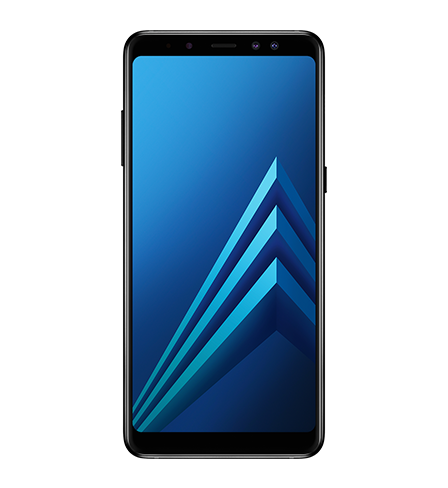
\includegraphics[width=\linewidth]{imgs/phone}
  \column{0.3\textwidth}
    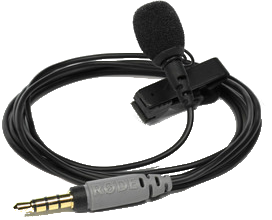
\includegraphics[width=\linewidth]{imgs/mic}
  \column{0.3\textwidth}
    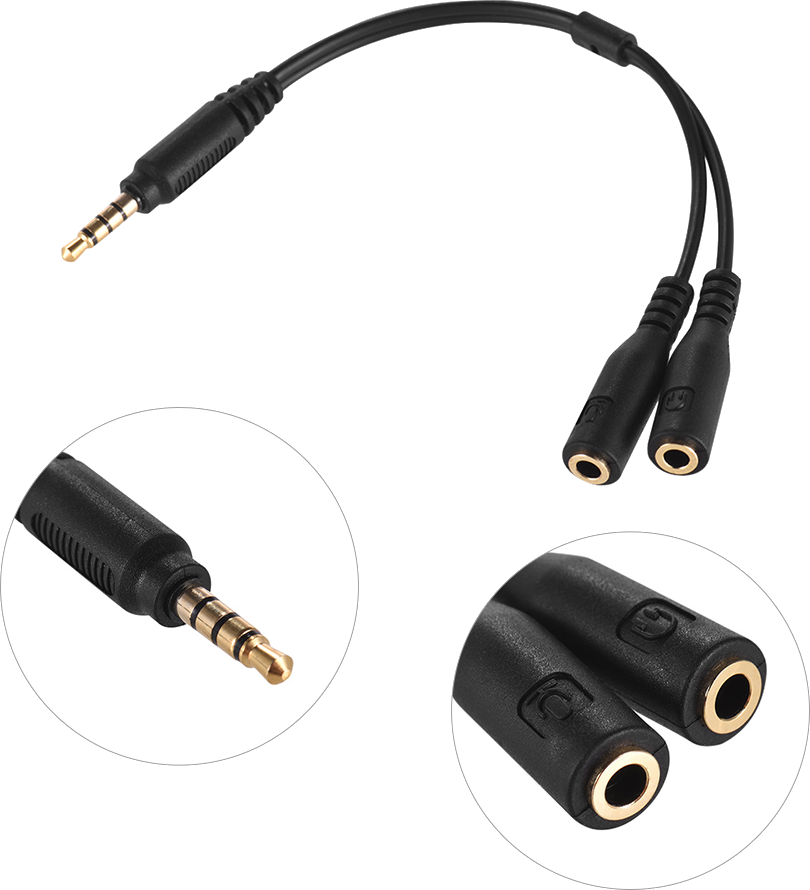
\includegraphics[width=\linewidth]{imgs/trrs}
\end{columns}
\end{frame}

\begin{frame}{External mic (iPhone)}
  \centering
  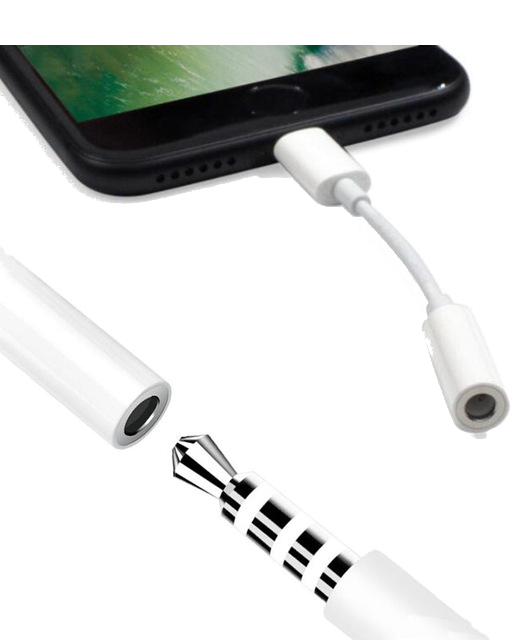
\includegraphics[width=0.4\linewidth]{imgs/35mm}
\end{frame}

\begin{frame}{Automatic Call Recorder Pro}
  Record phone calls

  \begin{figure}
    \centering
    
\includegraphics[width=0.25\linewidth]{imgs/acrp}\\
    \href{https://play.google.com/store/apps/details?id=com.appstar.callrecorderpro}{Google
  Play \beamergotobutton{Link}}
  \end{figure}

\end{frame}


\begin{frame}[fragile]{Noise removal}
  Using Audacity on your computer:
  \begin{enumerate}
    \item Open your audio file in Audacity.
    \item Select a pure noise area of the audio track.
    \item Open the \texttt{Effect / Noise reduction} menu.
    \item Click \texttt{Get Noise Profile}.
    \item Select the entire audio track.
    \item Open the \texttt{Effect / Noise reduction} menu again.
    \item Clik \texttt{OK} to apply the filter.
  \end{enumerate}
\end{frame}


\begin{frame}{Smart Doc Scanner}
  Digitise documents, straighten edges, OCR, full-text search

  \begin{figure}
  \centering
  
\includegraphics[width=0.3\linewidth]{imgs/sds}

  \href{https://www.youtube.com/watch?v=zAcMvZpTeBo}{YouTube \beamergotobutton{Link}}

  \href{https://play.google.com/store/apps/details?id=com.mobilicy.docscanner}{Google
  Play \beamergotobutton{Link}}
  \end{figure}

\end{frame}

\begin{frame}{PhotoSphere}

  \begin{itemize}
    \item Take multiple pictures
    \item Merge them together
    \item Allow to pan and zoom  \href{https://www.youtube.com/watch?v=zAcMvZpTeBo}{YouTube \beamergotobutton{Link}}

  \href{https://play.google.com/store/apps/details?id=com.mobilicy.docscanner}{Google
  Play \beamergotobutton{Link}}

  \end{itemize}

  \centering

  \begin{figure}
  
\includegraphics[width=0.3\linewidth]{imgs/photosphere}
  \end{figure}

  \href{https://www.youtube.com/watch?v=NPs3eIiWRaw}{YouTube \beamergotobutton{Link}}

  \href{https://g.co/photosphere}{g.co/photosphere \beamergotobutton{Link}}

\end{frame}

\begin{frame}{Version control}
  \small
  \begin{itemize}
    \item Management of changes to documents
    \item Version control systems allow collaboration
    \item \emph{Git} is the best one available
    \item Not very friendly
    \item Some applications to make it easier
     \begin{itemize}
       \item Source Tree \url{https://www.sourcetreeapp.com/}
     \end{itemize}
    \item \url{https://www.rithmschool.com/courses/git}
    \item \url{https://rogerdudler.github.io/git-guide/}
  \end{itemize}
\end{frame}

\begin{frame}{Privacy and security}
  \small
  \begin{columns}
    \column{0.48\textwidth}
    \begin{itemize}
      \item Signal (messaging)
      \item Phone/laptop encryption
      \item Protonmail (email)
      \item LastPass/1Password (password managers)
    \end{itemize}
    \column{0.48\textwidth}
    \begin{itemize}
      \item Tails (operating system)
      \item Tor (anonimity network)
      \item Tor Browser / Brave (private browsing)
      \item NordVPN (private browsing)
    \end{itemize}
  \end{columns}

\end{frame}

\begin{frame}{Bigvu}
  Teleprompter and more
  \begin{figure}
    \centering
  
\includegraphics[width=0.3\linewidth]{imgs/bigvu}


  \href{https://www.youtube.com/watch?time_continue=2&v=-yqQnW5s70E}{YouTube \beamergotobutton{Link}}

  \href{https://play.google.com/store/apps/details?id=bigvu.com.reporter}{Google
  Play \beamergotobutton{Link}}
  \end{figure}
\end{frame}

\begin{frame}{Evernote}
  Type notes, to-do's, add handwritten notes, images, audio, web pages

  \begin{figure}
  \centering
  
\includegraphics[width=0.4\linewidth]{imgs/evernote}

  \href{https://play.google.com/store/apps/details?id=com.evernote}{Google
  Play \beamergotobutton{Link}}
  \end{figure}
\end{frame}

\begin{frame}{Lapse It}
Capture time-lapse and stop motion videos

  \begin{figure}
  \centering
  
\includegraphics[width=0.4\linewidth]{imgs/lapseit}

  \href{https://play.google.com/store/apps/details?id=com.ui.LapseIt}{Google
  Play \beamergotobutton{Link}}
  \end{figure}
\end{frame}

\begin{frame}{Photo Exif Editor}
View, modify and remove the Exif data of pictures

  \begin{figure}
  \centering
  
\includegraphics[width=0.3\linewidth]{imgs/peep}

  \href{https://play.google.com/store/apps/details?id=net.xnano.android.photoexifeditor}{Google
  Play \beamergotobutton{Link}}
  \end{figure}
\end{frame}

\begin{frame}{PhotoScan}
  Printed photo scanner

  \begin{figure}
  \centering
  
\includegraphics[width=0.3\linewidth]{imgs/photoscan2}

  \href{https://google.com/photos/scan/}{google.com/photos/scan/}
  \end{figure}
\end{frame}

\begin{frame}{Warning: App permissions}

  \begin{columns}
    \column{0.43\textwidth}
      \centering
      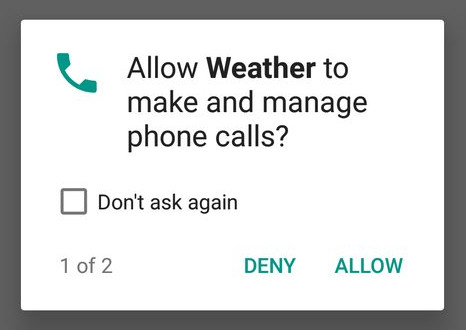
\includegraphics[width=\linewidth]{imgs/weather}
    \column{0.51\textwidth}
      \centering
      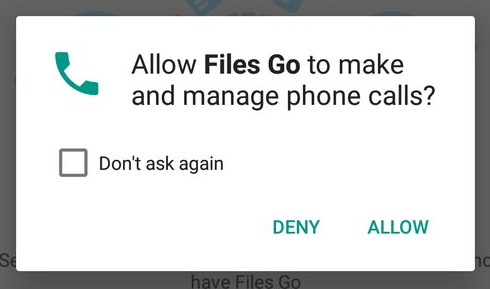
\includegraphics[width=\linewidth]{imgs/filesgo}
  \end{columns}
\end{frame}

\begin{frame}{Bouncer}
  Grant temporary permissions to other apps

  \begin{figure}
  \centering
  
\includegraphics[width=0.4\linewidth]{imgs/bouncer}

  \href{https://play.google.com/store/apps/details?id=com.samruston.permission}{Google
  Play \beamergotobutton{Link}}
  \end{figure}

\end{frame}


\begin{frame}{Slides}
Available at:
\begin{block}{~}
  \url{http://goo.gl/7P4oUN}
\end{block}
\end{frame}

\end{document}


